\begin{figure}[h!]
\includegraphics[width=\textwidth]{regions/out/regions.png}
\centering
\caption{\textbf{Summary statistics of disorder and order regions.}
\textbf{(A)} Distribution of mean lengths of regions.
\textbf{(B)} Violin plot of the sums of the average amino acid and indel substitution rates in the disorder and order regions. The substitution rates are significantly greater in the disorder regions than in the order regions ($p < 1 \times 10^{-10}$, Mann-Whitney \textit{U} test).}
\label{sfig:regions}
\end{figure}

\begin{figure}[h!]
\includegraphics[width=\textwidth]{pfam/out/pfam.png}
\centering
\caption{\textbf{Overlap of disorder and order regions with Pfam domains.}
\textbf{(A)} Number of disorder and order regions with zero and non-zero overlap with any Pfam domain. The proportion of regions with no overlap is significantly greater for the disorder regions ($p < 1 \times 10^{-10}$, chi-squared test).
\textbf{(B)} Histogram of the disorder and order regions' overlaps with any Pfam domain. Regions with zero overlap are excluded to more clearly show the distribution.}
\label{sfig:pfam}
\end{figure}

\begin{figure}[h!]
\includegraphics[width=\textwidth]{substitution/out/heatmap_ematrix.png}
\centering
\caption{\textbf{Exchangeability matrices fit to meta-alignments yielded by different sampling strategies.}
Each panel is a mean of the exchangeability coefficients fit to the meta-alignments yielded by a single sampling strategy ($n = 25$). The prefix and suffix in the title of each panel indicate the maximum gap fraction and region type of the columns in the meta-alignments, respectively. For example, the columns in the ``50R\_disorder'' set of meta-alignments were fewer than 50\% gaps and sampled from the disorder regions.}
\label{sfig:heatmap_ematrix}
\end{figure}

\begin{figure}[h!]
\includegraphics[width=\textwidth]{substitution/out/heatmap_rmatrix.png}
\centering
\caption{\textbf{Rate matrices fit to meta-alignments yielded by different sampling strategies.}
Each panel is a mean of the rate coefficients fit to the meta-alignments yielded by a single sampling strategy ($n = 25$). See \ref{sfig:heatmap_ematrix}~Fig for an explanation of the panel labels.}
\label{sfig:heatmap_rmatrix}
\end{figure}

\begin{figure}[h!]
\includegraphics[width=\textwidth]{substitution/out/heatmap_corr.png}
\centering
\caption{\textbf{Correlations between mean exchangeability and rate matrices fit to meta-alignments yielded by different sampling strategies.}
\textbf{(A)} Correlations between the mean exchangeability matrices in \ref{sfig:heatmap_ematrix}~Fig.
\textbf{(B)} Correlations between the mean rate matrices in \ref{sfig:heatmap_rmatrix}~Fig.}
\label{sfig:heatmap_corr}
\end{figure}

\begin{figure}[h!]
\includegraphics[width=\textwidth]{substitution/out/CV_ematrix.png}
\centering
\caption{\textbf{Coefficients of variation of the exchangeability matrices.}
For all panels, the top and bottoms rows correspond to the 50R\_disorder and 50R\_order meta-alignment sets, respectively.
\textbf{(A, D)} Mean exchangeability matrices.
\textbf{(B, E)} Coefficients of variation (ratio of the standard deviation to the mean) of exchangeability matrices.
\textbf{(C, F)} The coefficient of variation is inversely proportional to the mean, indicating the variation in the parameter estimates is constant relative to their magnitude.}
\label{sfig:CV_ematrix}
\end{figure}

\begin{figure}[h!]
\includegraphics[width=\textwidth]{substitution/out/CV_rmatrix.png}
\centering
\caption{\textbf{Coefficients of variation of the rate matrices.}
For all panels, the top and bottoms rows correspond to the 50R\_disorder and 50R\_order meta-alignment sets, respectively.
\textbf{(A, D)} Mean rate matrices.
\textbf{(B, E)} Coefficients of variation (ratio of the standard deviation to the mean) of rate matrices.
\textbf{(C, F)} The coefficient of variation is inversely proportional to the mean, indicating the variation in the parameter estimates is constant relative to their magnitude.}
\label{sfig:CV_rmatrix}
\end{figure}

\begin{figure}[h!]
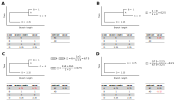
\includegraphics[width=\textwidth]{contrasts/out/contrasts.png}
\centering
\caption{\textbf{Sample contrasts calculation.}
\textbf{(A)} Initial state of tree with three tips. Values of traits at each tip are indicated on the tree and in the table.
\textbf{(B)} Calculation of first contrast between tips B and C.
\textbf{(C)} Inference of trait value at internal node A. Its branch length is increased to account for the uncertainty in the estimation of its value.
\textbf{(D)} Calculation of second contrast between tip D and internal node A.}
\label{sfig:contrasts}
\end{figure}

\begin{figure}[h!]
\includegraphics[width=0.75\textwidth]{scores/out/scores_histogram.png}
\centering
\caption{\textbf{Histogram of disorder score rates in regions.}
The grey interval indicates the upper decile of the distribution across both disorder and order regions, which was used as the input set for the GO term enrichment analysis.}
\label{sfig:scores_histogram}
\end{figure}

\begin{figure}[h!]
\includegraphics[width=\textwidth]{brownian/out/root_variance.png}
\centering
\caption{\textbf{Variance ratios of disorder regions' feature roots.}
\textbf{(A)} Variance ratios before normalization.
\textbf{(B)} Variance ratios after normalization.
\textbf{(C)} Scree plot of the explained variance ratio by PC.}
\label{sfig:root_variance}
\end{figure}

\begin{figure}[h!]
\includegraphics[width=\textwidth]{brownian/out/rate_variance.png}
\centering
\caption{\textbf{Variance ratios of disorder regions' feature rates.}
\textbf{(A)} Variance ratios before normalization.
\textbf{(B)} Variance ratios after normalization.
\textbf{(C)} Scree plot of the explained variance ratio by PC.}
\label{sfig:rate_variance}
\end{figure}

\begin{figure}[h!]
\includegraphics[width=\textwidth]{brownian/out/root.png}
\centering
\caption{\textbf{PCA of disorder regions' feature roots.}
\textbf{(A)} The first two PCs of the disorder regions' feature root distributions. The explained variance percentage of each component is indicated in parentheses in the axis labels.
\textbf{(B)} The same plot as panel A with the projections of original variables onto the components shown as arrows. Only the 16 features with the largest projections are shown. Scaling of the arrows is arbitrary.}
\label{sfig:root}
\end{figure}

\begin{figure}[h!]
\includegraphics[width=\textwidth]{brownian/out/order.png}
\centering
\caption{\textbf{PCA of order regions' feature rates.}
\textbf{(A)} The second and third PCs of the order regions' feature rate distributions. The explained variance percentage of each component is indicated in parentheses in the axis labels.
\textbf{(B)} The same plot as panel B with the projections of original variables onto the components shown as arrows. Only the 16 features with the largest projections are shown. Scaling of the arrows is arbitrary.}
\label{sfig:order}
\end{figure}

\begin{figure}[h!]
\includegraphics[width=\textwidth]{hierarchy/out/hierarchy_histogram.png}
\centering
\caption{\textbf{Rate distributions of substitution models fit to disorder regions.}
\textbf{(A)} Average amino acid rates in regions.
\textbf{(B)} Average indel rates in regions. For both panels, the grey intervals correspond to the subsets of rapidly evolving regions used for the clustering and GO term enrichment analyses. 5892 (52\%) and 6052 (53\%) regions pass the amino acid and indel rate cutoffs, respectively, and 7607 (67\%) of regions pass either.}
\label{sfig:hierarchy_histogram}
\end{figure}

\clearpage  % Force display of all figures before table

\begin{table}[h!]
\centering
\caption{\textbf{Phylogenetic diversity criteria.}}
\label{stable:diversity_criteria}
\begin{tabular}{|l|l|}
\hline
\textbf{Species IDs}   & \textbf{Minimum number}   \\ \hline
dinn,   dgri, dhyd     & 2                         \\ \hline
dnov,   dvir           & 1                         \\ \hline
dmoj,   dnav           & 1                         \\ \hline
dper,   dpse           & 1                         \\ \hline
dgua,   dsob           & 1                         \\ \hline
dana,   dbip           & 1                         \\ \hline
dkik,   dser           & 1                         \\ \hline
dele,   drho           & 1                         \\ \hline
dtak,   dbia           & 1                         \\ \hline
dspu,   dsuz           & 1                         \\ \hline
dere,   dtei           & 1                         \\ \hline
dsan,   dyak           & 1                         \\ \hline
dmel                   & 1                         \\ \hline
dmau,   dsec, dsim     & 1                         \\ \hline
\end{tabular}
\end{table}

\begin{landscape}
\footnotesize
\begin{longtable}{|l|l|l|l|l|l|}
\caption{\textbf{Features and their definitions.}}
\label{stable:features}
% Start first head
\\ \hline
\textbf{Feature ID}    & \textbf{Feature name}                                                            & \textbf{Group name}                                                & \textbf{Range} & \textbf{Description}                                                                                                             & \begin{tabular}[c]{@{}l@{}}\textbf{Changes from}\\\textbf{Zarin \textit{et al.}}~\cite{Zarin2019}\end{tabular}
\endfirsthead

% Start head
\multicolumn{6}{l}
{\textbf{\tablename\ \thetable} (continued)}
\\ \hline
\textbf{Feature ID}    & \textbf{Feature name}                                                            & \textbf{Group name}                                                & \textbf{Range} & \textbf{Description}                                                                                                             & \begin{tabular}[c]{@{}l@{}}\textbf{Changes from}\\\textbf{Zarin \textit{et al.}~\cite{Zarin2019}}\end{tabular}
\endhead

% Start foot
\multicolumn{6}{|c|}{Continued on next page}
\\ \hline
\endfoot

% Start last foot
\endlastfoot

\hline
fraction\_S            & S fraction                                                                       & \begin{tabular}[c]{@{}l@{}}amino acid\\content\end{tabular}        & {[}0, 1]                     &                                                                                                                                  &                                                                                                \\
\hline
fraction\_P            & P fraction                                                                       & \begin{tabular}[c]{@{}l@{}}amino acid\\content\end{tabular}        & {[}0, 1]                     &                                                                                                                                  &                                                                                                \\
\hline
fraction\_T            & T fraction                                                                       & \begin{tabular}[c]{@{}l@{}}amino acid\\content\end{tabular}        & {[}0, 1]                     &                                                                                                                                  &                                                                                                \\
\hline
fraction\_A            & A fraction                                                                       & \begin{tabular}[c]{@{}l@{}}amino acid\\content\end{tabular}        & {[}0, 1]                     &                                                                                                                                  &                                                                                                \\
\hline
fraction\_H            & H fraction                                                                       & \begin{tabular}[c]{@{}l@{}}amino acid\\content\end{tabular}        & {[}0, 1]                     &                                                                                                                                  &                                                                                                \\
\hline
fraction\_Q            & Q fraction                                                                       & \begin{tabular}[c]{@{}l@{}}amino acid\\content\end{tabular}        & {[}0, 1]                     &                                                                                                                                  &                                                                                                \\
\hline
fraction\_N            & N fraction                                                                       & \begin{tabular}[c]{@{}l@{}}amino acid\\content\end{tabular}        & {[}0, 1]                     &                                                                                                                                  &                                                                                                \\
\hline
fraction\_G            & G fraction                                                                       & \begin{tabular}[c]{@{}l@{}}amino acid\\content\end{tabular}        & {[}0, 1]                     &                                                                                                                                  &                                                                                                \\
\hline
FCR                    & \begin{tabular}[c]{@{}l@{}}fraction charged\\residues\end{tabular}               & \begin{tabular}[c]{@{}l@{}}charge\\properties\end{tabular}         & {[}0, 1]                     & basic residue fraction + acidic residue fraction                                                                                 &                                                                                                \\
\hline
NCPR                   & \begin{tabular}[c]{@{}l@{}}net charge\\per residue\end{tabular}                  & \begin{tabular}[c]{@{}l@{}}charge\\properties\end{tabular}         & {[}-1, 1]                    & basic residue fraction - acidic residue fraction                                                                                 &                                                                                                \\
\hline
net\_charge            & net charge                                                                       & \begin{tabular}[c]{@{}l@{}}charge\\properties\end{tabular}         & ($-\infty$, $\infty$)        & \#{[}RK] - \#{[}DE]                                                                                                              &                                                                                                \\
\hline
net\_charge\_P         & \begin{tabular}[c]{@{}l@{}}net charge with\\phosphorylation\end{tabular}         & \begin{tabular}[c]{@{}l@{}}charge\\properties\end{tabular}         & ($-\infty$, $\infty$)        & \begin{tabular}[c]{@{}l@{}}net charge including phosphorylation of [ST]P\\consensus sites with -1.5 charge per site\end{tabular} &                                                                                                \\
\hline
kappa                  & kappa                                                                            & \begin{tabular}[c]{@{}l@{}}charge\\properties\end{tabular}         & (0, 1]                       & \begin{tabular}[c]{@{}l@{}}measure of separation between positively\\and negatively charged residues\end{tabular}                &                                                                                                \\
\hline
omega                  & omega                                                                            & \begin{tabular}[c]{@{}l@{}}charge\\properties\end{tabular}         & (0, 1]                       & \begin{tabular}[c]{@{}l@{}}measure of separation between charged\\residues or prolines and all other residues\end{tabular}       &                                                                                                \\
\hline
SCD                    & \begin{tabular}[c]{@{}l@{}}sequence charge\\decoration\end{tabular}              & \begin{tabular}[c]{@{}l@{}}charge\\properties\end{tabular}         & ($-\infty$, $\infty$)        & \begin{tabular}[c]{@{}l@{}}measure of separation between positively\\and negatively charged residues\end{tabular}                &                                                                                                \\
\hline
RK\_ratio              & R/K ratio                                                                        & \begin{tabular}[c]{@{}l@{}}charge\\properties\end{tabular}         & (0, $\infty$)                & \begin{tabular}[c]{@{}l@{}}adjusted ratio of arginine to\\lysine residues: (\#R + 1)/(\#K + 1)\end{tabular}                      &                                                                                                \\
\hline
ED\_ratio              & E/D ratio                                                                        & \begin{tabular}[c]{@{}l@{}}charge\\properties\end{tabular}         & (0, $\infty$)                & \begin{tabular}[c]{@{}l@{}}adjusted ratio of glutamic acid to\\aspartic acid residues: (\#E + 1)/(\#D + 1)\end{tabular}          &                                                                                                \\
\hline
fraction\_acidic       & \begin{tabular}[c]{@{}l@{}}acidic\\residue fraction~\end{tabular}                & \begin{tabular}[c]{@{}l@{}}physiochemical\\properties\end{tabular} & {[}0 ,1]                     &                                                                                                                                  &                                                                                                \\
\hline
fraction\_basic        & \begin{tabular}[c]{@{}l@{}}basic\\residue fraction\end{tabular}                  & \begin{tabular}[c]{@{}l@{}}physiochemical\\properties\end{tabular} & {[}0 ,1]                     &                                                                                                                                  &                                                                                                \\
\hline
fraction\_aliphatic    & \begin{tabular}[c]{@{}l@{}}aliphatic\\residue fraction\end{tabular}              & \begin{tabular}[c]{@{}l@{}}physiochemical\\properties\end{tabular} & {[}0 ,1]                     &                                                                                                                                  &                                                                                                \\
\hline
fraction\_polar        & \begin{tabular}[c]{@{}l@{}}polar\\residue fraction\end{tabular}                  & \begin{tabular}[c]{@{}l@{}}physiochemical\\properties\end{tabular} & {[}0 ,1]                     &                                                                                                                                  & removed glycine                                                                                \\
\hline
fraction\_chainexp     & \begin{tabular}[c]{@{}l@{}}chain-expanding\\residue fraction\end{tabular}        & \begin{tabular}[c]{@{}l@{}}physiochemical\\properties\end{tabular} & {[}0 ,1]                     &                                                                                                                                  &                                                                                                \\
\hline
fraction\_aromatic     & \begin{tabular}[c]{@{}l@{}}aromatic\\residue fraction\end{tabular}               & \begin{tabular}[c]{@{}l@{}}physiochemical\\properties\end{tabular} & {[}0 ,1]                     &                                                                                                                                  &                                                                                                \\
\hline
fraction\_disorder     & \begin{tabular}[c]{@{}l@{}}disorder-promoting\\residue fraction\end{tabular}     & \begin{tabular}[c]{@{}l@{}}physiochemical\\properties\end{tabular} & {[}0 ,1]                     &                                                                                                                                  &                                                                                                \\
\hline
radius\_gyration       & radius of gyration                                                               & \begin{tabular}[c]{@{}l@{}}physiochemical\\properties\end{tabular} & {[}0,~ $\infty$)             & number of residues to the 0.6 power                                                                                              & \begin{tabular}[c]{@{}l@{}}substituted\\for length\end{tabular}                                \\
\hline
hydropathy             & hydropathy                                                                       & \begin{tabular}[c]{@{}l@{}}physiochemical\\properties\end{tabular} & {[}0 ,1]                     & normalized Kyte-Doolittle scale                                                                                                  &                                                                                                \\
\hline
isopoint               & isoelectric point                                                                & \begin{tabular}[c]{@{}l@{}}physiochemical\\properties\end{tabular} & ($-\infty$, $\infty$)        & pH where charge of peptide is neutral                                                                                            &                                                                                                \\
\hline
PPII\_propensity       & PPII propensity                                                                  & \begin{tabular}[c]{@{}l@{}}physiochemical\\properties\end{tabular} & {[}0, 1]                     & \begin{tabular}[c]{@{}l@{}}propensity for proline to form\\left-handed helices\end{tabular}                                      &                                                                                                \\
\hline
repeat\_Q              & Q repeat fraction                                                                & \begin{tabular}[c]{@{}l@{}}repeats and\\complexity\end{tabular}    & {[}0, 1]                     & fraction 2 or more consecutive Q                                                                                                 &                                                                                                \\
\hline
repeat\_N              & N repeat fraction                                                                & \begin{tabular}[c]{@{}l@{}}repeats and\\complexity\end{tabular}    & {[}0, 1]                     & fraction 2 or more consecutive N                                                                                                 &                                                                                                \\
\hline
repeat\_S              & S repeat fraction                                                                & \begin{tabular}[c]{@{}l@{}}repeats and\\complexity\end{tabular}    & {[}0, 1]                     & fraction 2 or more consecutive S                                                                                                 &                                                                                                \\
\hline
repeat\_G              & G repeat fraction                                                                & \begin{tabular}[c]{@{}l@{}}repeats and\\complexity\end{tabular}    & {[}0, 1]                     & fraction 2 or more consectuive G                                                                                                 &                                                                                                \\
\hline
repeat\_E              & E repeat fraction                                                                & \begin{tabular}[c]{@{}l@{}}repeats and\\complexity\end{tabular}    & {[}0, 1]                     & fraction 2 or more consecutive E                                                                                                 &                                                                                                \\
\hline
repeat\_D              & D repeat fraction                                                                & \begin{tabular}[c]{@{}l@{}}repeats and\\complexity\end{tabular}    & {[}0, 1]                     & fraction 2 or more consecutive D                                                                                                 &                                                                                                \\
\hline
repeat\_K              & K repeat fraction                                                                & \begin{tabular}[c]{@{}l@{}}repeats and\\complexity\end{tabular}    & {[}0, 1]                     & fraction 2 or more consecutive K                                                                                                 &                                                                                                \\
\hline
repeat\_R              & R repeat fraction                                                                & \begin{tabular}[c]{@{}l@{}}repeats and\\complexity\end{tabular}    & {[}0, 1]                     & fraction 2 or more consecutive R                                                                                                 &                                                                                                \\
\hline
repeat\_P              & P repeat fraction                                                                & \begin{tabular}[c]{@{}l@{}}repeats and\\complexity\end{tabular}    & {[}0, 1]                     & fraction 2 or more consecutive P                                                                                                 &                                                                                                \\
\hline
repeat\_QN             & {[}QN] repeat fraction                                                           & \begin{tabular}[c]{@{}l@{}}repeats and\\complexity\end{tabular}    & {[}0, 1]                     & fraction 2 or more consecutive [QN]                                                                                              &                                                                                                \\
\hline
repeat\_RG             & {[}RG] repeat fraction                                                           & \begin{tabular}[c]{@{}l@{}}repeats and\\complexity\end{tabular}    & {[}0, 1]                     & fraction 2 or more consecutive [RG]                                                                                              &                                                                                                \\
\hline
repeat\_FG             & {[}FG] repeat fraction                                                           & \begin{tabular}[c]{@{}l@{}}repeats and\\complexity\end{tabular}    & {[}0, 1]                     & fraction 2 or more consecutive [FG]                                                                                              &                                                                                                \\
\hline
repeat\_SG             & {[}SG] repeat fraction                                                           & \begin{tabular}[c]{@{}l@{}}repeats and\\complexity\end{tabular}    & {[}0, 1]                     & fraction 2 or more consecutive [SG]                                                                                              &                                                                                                \\
\hline
repeat\_SR             & {[}SR] repeat fraction                                                           & \begin{tabular}[c]{@{}l@{}}repeats and\\complexity\end{tabular}    & {[}0, 1]                     & fraction 2 or more consecutive [SR]                                                                                              &                                                                                                \\
\hline
repeat\_AP             & {[}KAP] repeat fraction                                                          & \begin{tabular}[c]{@{}l@{}}repeats and\\complexity\end{tabular}    & {[}0, 1]                     & fraction 2 or more consecutive [KAP]                                                                                             &                                                                                                \\
\hline
repeat\_TS             & {[}PTS] repeat fraction                                                          & \begin{tabular}[c]{@{}l@{}}repeats and\\complexity\end{tabular}    & {[}0, 1]                     & fraction 2 or more consecutive [PTS]                                                                                             &                                                                                                \\
\hline
wf\_complexity         & \begin{tabular}[c]{@{}l@{}}Wootton-Federhen\\sequence complexity\end{tabular}    & \begin{tabular}[c]{@{}l@{}}repeats and\\complexity\end{tabular}    & {[}0, 1]                     & \begin{tabular}[c]{@{}l@{}}complexity based on SEG algorithm:\\blob length=IDR length, step size=1\end{tabular}                  &                                                                                                \\
\hline
CLV\_Separin\_Metazoa  & separase cleavage motif                                                          & motifs                                                             & {[}0, $\infty$)              &                                                                                                                                  & \begin{tabular}[c]{@{}l@{}}Metazoa motif\\instead of fungi\end{tabular}                        \\
\hline
DEG\_APCC\_KENBOX\_2   & \begin{tabular}[c]{@{}l@{}}APCC-binding\\destruction motif\end{tabular}          & motifs                                                             & {[}0, $\infty$)              &                                                                                                                                  &                                                                                                \\
\hline
DEG\_APCC\_TPR\_1      & APCC-TPR-docking motif                                                           & motifs                                                             & {[}0, $\infty$)              &                                                                                                                                  &                                                                                                \\
\hline
DOC\_CKS1\_1           & Cks1 ligand                                                                      & motifs                                                             & {[}0, $\infty$)              &                                                                                                                                  &                                                                                                \\
\hline
DOC\_MAPK\_DCC\_7      & MAPK docking motif                                                               & motifs                                                             & {[}0, $\infty$)              &                                                                                                                                  &                                                                                                \\
\hline
DOC\_MAPK\_gen\_1      & MAPK docking motif                                                               & motifs                                                             & {[}0, $\infty$)              &                                                                                                                                  &                                                                                                \\
\hline
DOC\_MAPK\_HePTP\_8    & MAPK docking motif                                                               & motifs                                                             & {[}0, $\infty$)              &                                                                                                                                  &                                                                                                \\
\hline
DOC\_PP1\_RVXF\_1      & PP1-docking motif RVXF                                                           & motifs                                                             & {[}0, $\infty$)              &                                                                                                                                  &                                                                                                \\
\hline
DOC\_PP2B\_PxIxI\_1    & \begin{tabular}[c]{@{}l@{}}calcineurin (PP2B)-\\docking motif PxIxI\end{tabular} & motifs                                                             & {[}0, $\infty$)              &                                                                                                                                  &                                                                                                \\
\hline
LIG\_APCC\_Cbox\_1     & \begin{tabular}[c]{@{}l@{}}APC/C\_Apc2-docking\\motif\end{tabular}               & motifs                                                             & {[}0, $\infty$)              &                                                                                                                                  & \begin{tabular}[c]{@{}l@{}}Metazoa motif\\instead of fungi\end{tabular}                        \\
\hline
LIG\_AP\_GAE\_1        & \begin{tabular}[c]{@{}l@{}}gamma-adaptin ear\\interaction motif\end{tabular}     & motifs                                                             & {[}0, $\infty$)              &                                                                                                                                  &                                                                                                \\
\hline
LIG\_CaM\_IQ\_9        & \begin{tabular}[c]{@{}l@{}}helical calmodulin\\binding motif\end{tabular}        & motifs                                                             & {[}0, $\infty$)              &                                                                                                                                  &                                                                                                \\
\hline
LIG\_EH\_1             & EH ligand                                                                        & motifs                                                             & {[}0, $\infty$)              &                                                                                                                                  &                                                                                                \\
\hline
LIG\_eIF4E\_1          & eIF4E binding motif                                                              & motifs                                                             & {[}0, $\infty$)              &                                                                                                                                  &                                                                                                \\
\hline
LIG\_GLEBS\_BUB3\_1    & GLEBS motif                                                                      & motifs                                                             & {[}0, $\infty$)              &                                                                                                                                  &                                                                                                \\
\hline
LIG\_LIR\_Gen\_1       & \begin{tabular}[c]{@{}l@{}}Atg8 protein\\family ligands\end{tabular}             & motifs                                                             & {[}0, $\infty$)              &                                                                                                                                  & \begin{tabular}[c]{@{}l@{}}same ELM entry,\\but updated regex\end{tabular}                     \\
\hline
LIG\_PCNA\_PIPBox\_1   & PCNA binding PIP box                                                             & motifs                                                             & {[}0, $\infty$)              &                                                                                                                                  & \begin{tabular}[c]{@{}l@{}}same ELM entry,\\but updated regex\end{tabular}                     \\
\hline
LIG\_SUMO\_SIM\_par\_1 & \begin{tabular}[c]{@{}l@{}}SUMO interaction\\site\end{tabular}                   & motifs                                                             & {[}0, $\infty$)              &                                                                                                                                  &                                                                                                \\
\hline
MOD\_CDK\_SPxK\_1      & \begin{tabular}[c]{@{}l@{}}CDK phosphorylation\\site\end{tabular}                & motifs                                                             & {[}0, $\infty$)              &                                                                                                                                  &                                                                                                \\
\hline
MOD\_LATS\_1           & \begin{tabular}[c]{@{}l@{}}LATS kinase\\phosphorylation motif\end{tabular}       & motifs                                                             & {[}0, $\infty$)              &                                                                                                                                  &                                                                                                \\
\hline
MOD\_SUMO\_for\_1      & sumoylation site                                                                 & motifs                                                             & {[}0, $\infty$)              &                                                                                                                                  &                                                                                                \\
\hline
TRG\_ER\_FFAT\_1       & FFAT motif                                                                       & motifs                                                             & {[}0, $\infty$)              &                                                                                                                                  & \begin{tabular}[c]{@{}l@{}}same ELM entry,\\but updated regex\end{tabular}                     \\
\hline
TRG\_Golgi\_diPhe\_1   & ER export signals                                                                & motifs                                                             & {[}0, $\infty$)              &                                                                                                                                  &                                                                                                \\
\hline
TRG\_NLS\_MonoExtN\_4  & \begin{tabular}[c]{@{}l@{}}classical nuclear\\localization signals\end{tabular}  & motifs                                                             & {[}0, $\infty$)              &                                                                                                                                  &                                                                                                \\
\hline
MOD\_CDK\_STP          & \begin{tabular}[c]{@{}l@{}}CDK phosphorylation\\motif\end{tabular}               & motifs                                                             & {[}0, $\infty$)              &                                                                                                                                  &                                                                                                \\
\hline
MOD\_MEC1              & \begin{tabular}[c]{@{}l@{}}Mec1 phosphorylation\\motif\end{tabular}              & motifs                                                             & {[}0, $\infty$)              &                                                                                                                                  &                                                                                                \\
\hline
MOD\_PRK1              & \begin{tabular}[c]{@{}l@{}}Prk1 phosphorylation\\motif\end{tabular}              & motifs                                                             & {[}0, $\infty$)              &                                                                                                                                  &                                                                                                \\
\hline
MOD\_IPL1              & \begin{tabular}[c]{@{}l@{}}Ipl1 phosphorylation\\motif\end{tabular}              & motifs                                                             & {[}0, $\infty$)              &                                                                                                                                  &                                                                                                \\
\hline
MOD\_PKA               & \begin{tabular}[c]{@{}l@{}}Pka phosphorylation\\motif\end{tabular}               & motifs                                                             & {[}0, $\infty$)              &                                                                                                                                  &                                                                                                \\
\hline
MOD\_CKII              & \begin{tabular}[c]{@{}l@{}}Ckii phosphorylation\\motif\end{tabular}              & motifs                                                             & {[}0, $\infty$)              &                                                                                                                                  &                                                                                                \\
\hline
MOD\_IME2              & \begin{tabular}[c]{@{}l@{}}Ime2 phosphorylation\\motif\end{tabular}              & motifs                                                             & {[}0, $\infty$)              &                                                                                                                                  &                                                                                                \\
\hline
DOC\_PRO               & proline rich motif                                                               & motifs                                                             & {[}0, $\infty$)              &                                                                                                                                  &                                                                                                \\
\hline
TRG\_ER\_HDEL          & ER localization motif                                                            & motifs                                                             & {[}0, $\infty$)              &                                                                                                                                  &                                                                                                \\
\hline
TRG\_MITOCHONDRIA      & \begin{tabular}[c]{@{}l@{}}mitochondrial\\localization motif\end{tabular}        & motifs                                                             & {[}0, $\infty$)              &                                                                                                                                  &                                                                                                \\
\hline
MOD\_ISOMERASE         & \begin{tabular}[c]{@{}l@{}}disulfide isomerase\\motif\end{tabular}               & motifs                                                             & {[}0, $\infty$)              &                                                                                                                                  &                                                                                                \\
\hline
TRG\_FG                & \begin{tabular}[c]{@{}l@{}}FG nucleoporin\\motif\end{tabular}                    & motifs                                                             & {[}0, $\infty$)              &                                                                                                                                  &                                                                                                \\
\hline
INT\_RGG               & RGG motif                                                                        & motifs                                                             & {[}0, $\infty$)              &                                                                                                                                  &                                                                                                \\
\hline
\end{longtable}
\end{landscape}

\begin{landscape}
\footnotesize
\begin{longtable}{|l|l|}
\caption{\textbf{Feature regular expressions.}}
\label{stable:regexes}
% Start first head
\\ \hline
\textbf{Feature ID}    & \textbf{Regular expression}
\endfirsthead

% Start head
\multicolumn{2}{l}
{\textbf{\tablename\ \thetable} (continued)}
\\ \hline
\textbf{Feature ID}    & \textbf{Regular expression}
\endhead

% Start foot
\multicolumn{2}{|c|}{Continued on next page}
\\ \hline
\endfoot

% Start last foot
\endlastfoot

\hline
fraction\_S            & S                                                                                                                          \\
\hline
fraction\_P            & P                                                                                                                          \\
\hline
fraction\_T            & T                                                                                                                          \\
\hline
fraction\_A            & A                                                                                                                          \\
\hline
fraction\_H            & H                                                                                                                          \\
\hline
fraction\_Q            & Q                                                                                                                          \\
\hline
fraction\_N            & N                                                                                                                          \\
\hline
fraction\_G            & G                                                                                                                          \\
\hline
fraction\_acidic       & {[}DE]                                                                                                                     \\
\hline
fraction\_basic        & {[}RK]                                                                                                                     \\
\hline
fraction\_aliphatic    & {[}ALMIV]                                                                                                                  \\
\hline
fraction\_polar        & {[}QNSTCH]                                                                                                                 \\
\hline
fraction\_chainexp     & {[}EDRKP]                                                                                                                  \\
\hline
fraction\_aromatic     & {[}FYW]                                                                                                                    \\
\hline
fraction\_disorder     & {[}TAGRDHQKSEP]                                                                                                            \\
\hline
repeat\_Q              & Q\{2,\}                                                                                                                    \\
\hline
repeat\_N              & N\{2,\}                                                                                                                    \\
\hline
repeat\_S              & S\{2,\}                                                                                                                    \\
\hline
repeat\_G              & G\{2,\}                                                                                                                    \\
\hline
repeat\_E              & E\{2,\}                                                                                                                    \\
\hline
repeat\_D              & D\{2,\}                                                                                                                    \\
\hline
repeat\_K              & K\{2,\}                                                                                                                    \\
\hline
repeat\_R              & R\{2,\}                                                                                                                    \\
\hline
repeat\_P              & P\{2,\}                                                                                                                    \\
\hline
repeat\_QN             & {[}QN]\{2,\}                                                                                                               \\
\hline
repeat\_RG             & {[}RG]\{2,\}                                                                                                               \\
\hline
repeat\_FG             & {[}FG]\{2,\}                                                                                                               \\
\hline
repeat\_SG             & {[}SG]\{2,\}                                                                                                               \\
\hline
repeat\_SR             & {[}SR]\{2,\}                                                                                                               \\
\hline
repeat\_AP             & {[}KAP]\{2,\}                                                                                                              \\
\hline
repeat\_TS             & {[}PTS]\{2,\}                                                                                                              \\
\hline
CLV\_Separin\_Metazoa  & E[IMPVL][MLVP]R.                                                                                                           \\
\hline
DEG\_APCC\_KENBOX\_2   & .KEN.                                                                                                                      \\
\hline
DEG\_APCC\_TPR\_1      & .[ILM]R                                                                                                                    \\
\hline
DOC\_CKS1\_1           & {[}MPVLIFWYQ].(T)P..                                                                                                       \\
\hline
DOC\_MAPK\_DCC\_7      & {[}RK].\{2,4\}{[}LIVP]P.[LIV].[LIVMF]\textbar{}{[}RK].\{2,4\}{[}LIVP].P[LIV].[LIVMF]                                       \\
\hline
DOC\_MAPK\_gen\_1      & {[}KR]\{0,2\}{[}KR].\{0,2\}{[}KR].\{2,4\}{[}ILVM].[ILVF]                                                                   \\
\hline
DOC\_MAPK\_HePTP\_8    & ([LIV][\^{}P][\^{}P][RK]....[LIVMP].[LIV].[LIVMF])\textbar{}([LIV][\^{}P][\^{}P][RK][RK]G.\{4,7\}{[}LIVMP].[LIV].[LIVMF])  \\
\hline
DOC\_PP1\_RVXF\_1      & ..[RK].\{0,1\}{[}VIL][\^{}P][FW].                                                                                          \\
\hline
DOC\_PP2B\_PxIxI\_1    & .P[\^{}P]I[\^{}P][IV][\^{}P]                                                                                               \\
\hline
LIG\_APCC\_Cbox\_1     & {[}DE]R[YFH][ILFVM][PAG].R                                                                                                 \\
\hline
LIG\_AP\_GAE\_1        & {[}DE][DES][DEGAS]F[SGAD][DEAP][LVIMFD]                                                                                    \\
\hline
LIG\_CaM\_IQ\_9        & {[}ACLIVTM][\^{}P][\^{}P][ILVMFCT]Q[\^{}P][\^{}P][\^{}P][RK][\^{}P]\{4,5\}{[}RKQ][\^{}P][\^{}P]                            \\
\hline
LIG\_EH\_1             & .NPF.                                                                                                                      \\
\hline
LIG\_eIF4E\_1          & Y....L[VILMF]                                                                                                              \\
\hline
LIG\_GLEBS\_BUB3\_1    & {[}EN][FYLW][NSQ].EE[ILMVF][\^{}P][LIVMFA]                                                                                 \\
\hline
LIG\_LIR\_Gen\_1       & {[}EDST].\{0,2\}{[}WFY][\^{}RKPGWFY][\^{}PG][ILVFM]((.\{0,4\}{[}PLAFIVMY])\textbar{}(\$)\textbar{}(.\{0,3\}{[}ED]))        \\
\hline
LIG\_PCNA\_PIPBox\_1   & {[}QM].[\^{}FHWY][LIVM][\^{}P][\^{}PFWYMLIV](([FYHL][FYW])\textbar{}([FYH][FYWL]))..                                       \\
\hline
LIG\_SUMO\_SIM\_par\_1 & {[}DEST]\{0,5\}.[VILPTM][VIL][DESTVILMA][VIL].\{0,1\}{[}DEST]\{1,10\}                                                      \\
\hline
MOD\_CDK\_SPxK\_1      & ...([ST])P.[KR]                                                                                                            \\
\hline
MOD\_LATS\_1           & H.[KR]..([ST])[\^{}P]                                                                                                      \\
\hline
MOD\_SUMO\_for\_1      & {[}VILMAFP](K).E                                                                                                           \\
\hline
TRG\_ER\_FFAT\_1       & {[}EDS].\{0,4\}{[}ED][FY][FYKREM][DE][AC].\{1,2\}{[}EDST]                                                                  \\
\hline
TRG\_Golgi\_diPhe\_1   & Q.\{6,6\}FF.\{6,7\}                                                                                                        \\
\hline
TRG\_NLS\_MonoExtN\_4  & (([PKR].\{0,1\}{[}\^{}DE])\textbar{}([PKR]))((K[RK])\textbar{}(RK))(([\^{}DE][KR])\textbar{}([KR][\^{}DE]))[\^{}DE]        \\
\hline
MOD\_CDK\_STP          & {[}ST]P                                                                                                                    \\
\hline
MOD\_MEC1              & {[}ST]Q                                                                                                                    \\
\hline
MOD\_PRK1              & {[}LIVM]....TG                                                                                                             \\
\hline
MOD\_IPL1              & {[}RK].[ST][LIV]                                                                                                           \\
\hline
MOD\_PKA               & R[RK].S                                                                                                                    \\
\hline
MOD\_CKII              & {[}ST][DE].[DE]                                                                                                            \\
\hline
MOD\_IME2              & RP.[ST]                                                                                                                    \\
\hline
DOC\_PRO               & P..P                                                                                                                       \\
\hline
TRG\_ER\_HDEL          & HDEL                                                                                                                       \\
\hline
TRG\_MITOCHONDRIA      & {[}MR]L[RK]                                                                                                                \\
\hline
MOD\_ISOMERASE         & C..C                                                                                                                       \\
\hline
TRG\_FG                & F.FG\textbar{}GLFG                                                                                                         \\
\hline
INT\_RGG               & RGG\textbar{}RG                                                                                                            \\
\hline
\end{longtable}
\end{landscape}
